\section*{Knowledge Checks}

\subsection*{Network Layer: Data plane}
    \subsubsection*{The network layer - where is it?}
    \noindent All the next statements about where (\textit{in the network}) the network layer is implemented are true
    \begin{itemize}
        \item The network layer is implemented in hosts at the network's edge.
        \item The network layer is implemented in routers in the network core.
    \end{itemize}

    \subsubsection*{Forwarding versus routing}
    \noindent Consider the travel analogy discussed in the textbook - some actions we take on a trip correspond to forwarding
    and other actions we take on a trip correspond to routing. The following travel actions correspond to \textit{forwarding}.
    \begin{itemize}
        \item A car stops at an intersection to "gas-up" and take a "bathroom break".
        \item A car waits at light and then returns left at the intersection.
        \item A car takes the 3rd exit from a roundabout. 
    \end{itemize}

    \noindent The following travel actions correspond to \textit{routing}
    \begin{itemize}
        \item A car takes highway 80 between New York and Chicago, rather than highway 87 to Albany and from there take
        interstate 90 to Chicago.
        \item A traveler decides to fly to Sydney through Singapore rather than Dubai.
        \item a climber decides to take the South Col Route to the top of Mt Everest rather than the Northeast Ridge route.
    \end{itemize}

    \subsubsection*{The control plane versus the data plane}
    \noindent The following actions are primarily in the network-layer data plane
    \begin{itemize}
        \item Looking up address bits in an arriving datagram header in the forwarding table.
        \item Dropping a datagram due to a congested (\textit{full}) output buffer.
        \item Moving an arriving datagram from a router's input port to output port.
    \end{itemize}

    \noindent The following actions correspond to contro-plane actions
    \begin{itemize}
        \item Monitoring and managing the configuration and performance if an network device.
        \item Computing the contents of the forwarding table.
    \end{itemize}

    \subsubsection*{What type of control plane?}
    \noindent We've seen that there are two approaches towards implementing the network control plane a per-router control-plane approach and a
    software-networking (\textit{SDN}) control-plane approach. The following actions occur in a per-router control-plane approach
    \begin{itemize}
        \item Routers send information about their incoming and outgoing links to other routers in the network.
        \item A router exchanges messages with another router, indicating the cost for it (\textit{the sending router}) to reach a destination host.
    \end{itemize}

    \noindent These actions correspond to actions in an SDN control plane
    \begin{itemize}
        \item All routers in the network send information about their incoming and outgoing links to a logically centralized controller.
        \item A control agent in router receives a complete forwarding table, which it installs and uses to locally control datagram forwarding.
    \end{itemize}

    \subsubsection*{Best Effort Service}
    \noindent The following quality-of-service guarantees are part of the Internet's best-effort service model
    \begin{itemize}
        \item The best-effort service really means no \textit{guarantees} at all!
    \end{itemize}

\subsection*{Network Layer: Control plane}
    \subsubsection*{What's a "good" path?}
    \noindent What is the definition of a "good" path for a routing protocol?
    Rounting algorithms typically work with abstract link weights that could represent any of, or combinations of, all of the other answers.

    \subsubsection*{Dijkstra's Link-State routing algorithm}
    \noindent Consider Dijkstra's link-state routing algorithm that is computing a least-cost path from a node a to other nodes b, c, d, e, f. The following
    statements are true
    \begin{itemize}
        \item The values computed in the vector D(v), the currently known least cost of a path from a to any node v, will never increase following in iteration.
        \item In the initilization step, the initial cost from a to each of these destinations is initialized to either the cost of a link directly connecting
        a to a direct neighbor, or infinity otherwise.
        \item Suppose node b, c and d are in the set N'. These nodes will remain in N' for the rest of the algorithm, since the least-cost paths from a to b, c,
        and d are known.
    \end{itemize}

    \subsubsection*{What type of routing?}
    \noindent Here are the names of a general approach to routing with characteristics of that approach
    \begin{description}
        \item[Centralized, global routing] - All routers have complete topology, and link cost information.
        \item[Decentralized routing] - An iterative process of computation, exchange of information with neighbors. Routers may initially only
        know link costs to directly-attached neighbors.
        \item[Static routing] - Routes change slowly over time.
        \item[Dynamic routing] - Rounting changes quickly over time.     
    \end{description}

    \subsubsection*{Dijkstra's link-state routing algorithm (\textit{Part 1})}
    \noindent Consider the graph shown below and the use of Dijkstra's algorithm to compute a least cost path a to all destinations. Suppose that nodes b and d have
    already been added to N'. What is the next node to be added to N' (\textit{refer to the text for an explanation of notation})? \textbf{The next node is e}
    \begin{figure}[H]
        \centering
        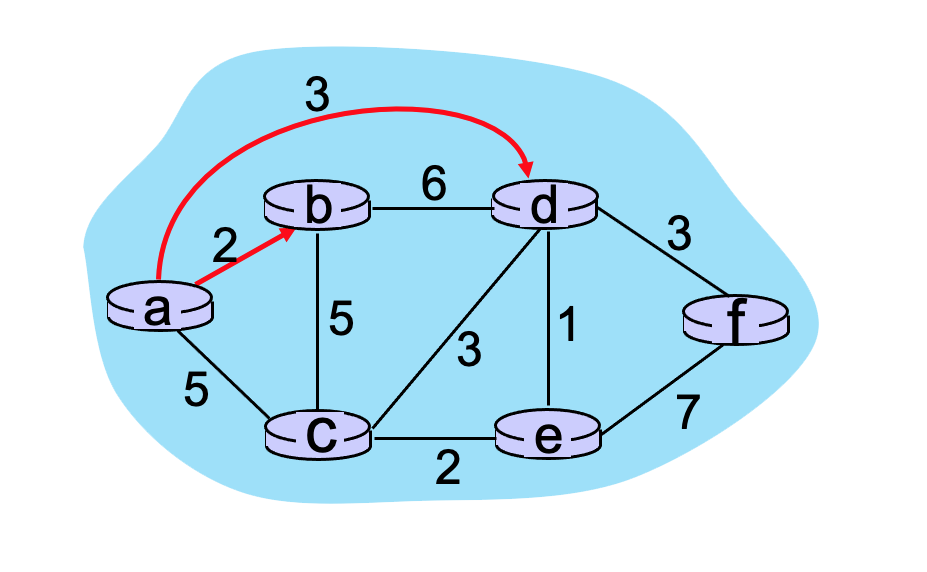
\includegraphics[width=0.6\textwidth]{img/Dijsktra_kc_network.png}
    \end{figure}

    \subsubsection*{Dijkstra's link-state routing algorithm (\textit{Part 2})}
    \noindent Consider the graph previously shown and the use of Dijkstra's algorithm to compute a least cost path from a to all destinations. Suppose that b and d have
    already been added to N'. What is the path cost to the next node to be added to N' (\textit{refer to the next for an explanation of notation})? \textbf{The path cost is 4}

    \subsubsection*{Dijkstra's link state algorithm (\textit{for computing least cost paths})}
    \noindent Consider the 6-node network shown below, with the given link costs. Using Dijkstra's algorithm, find the least cost path from source node U to all other
    destinations
    \begin{figure}[H]
        \centering
        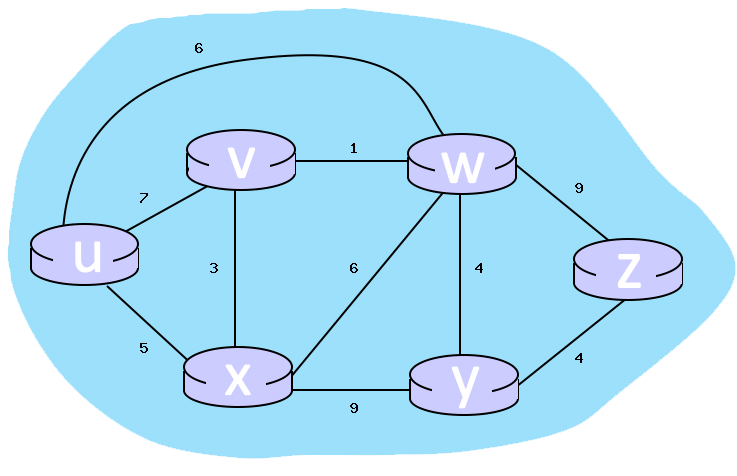
\includegraphics[width=0.6\textwidth]{img/descarga.png}
    \end{figure}
    \begin{description}
        \item[What is the shortest distance to node v and what node is its predecessor?] The answer is: 7, u.
        \item[What is the shortest distance to node y and what node is its predecessor?] The answer is: 10, w. 
        \item[What is the shortest distance to node w and what node is its predecessor?] The answer is: 6, u. 
    \end{description}

    \newpage
    \subsubsection*{Dijkstra's link state algorithm - advanced}
    \noindent Consider the incomplete 6-node network shown below, with the given link costs
    \begin{figure}[H]
        \centering
        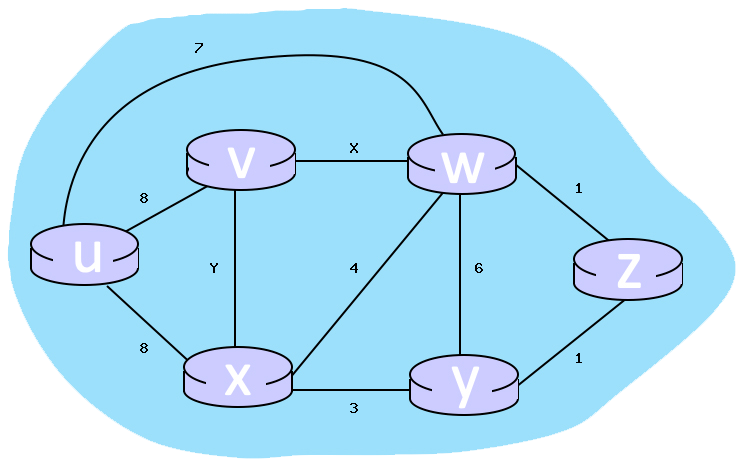
\includegraphics[width=0.6\textwidth]{img/descarga (1).png}
    \end{figure}

    \noindent Consider the completed table below, which calculates the shortest distance to all node from X:
    \begin{table}[H]
        \centering
        \begin{tabular}{@{}ccc@{}}
        \toprule
        \multicolumn{1}{l}{Node} & \begin{tabular}[c]{@{}c@{}}Shortest distance\\ from X\end{tabular} & Previous Node \\ \midrule
        X                        & 0                                                                  & n/a           \\
        Y                        & 3                                                                  & X             \\
        W                        & 4                                                                  & X             \\
        Z                        & 4                                                                  & Y             \\
        V                        & 7                                                                  & X             \\
        U                        & 8                                                                  & X             \\ \bottomrule
        \end{tabular}
    \end{table}

    \begin{description}
        \item[For link X, what is the cost associated with this link?] The answer is: n/a.
        \item[For link Y, what is the cost associated with this link?] The answer is: 7. 
    \end{description}

\subsection*{Link Layer}
    \subsubsection*{Link-layer services}
    \noindent The following services may be implemented in a link-layer protocol?
    \begin{itemize}
        \item Flow control between directly connected nodes.
        \item Multiplexing down from / mutiplexing up to a network-layer protocol.
        \item Reliable data transfer between directly connected nodes.
        \item Coordinated access to a shared physical medium.
        \item Bit-level error detection and correction.
    \end{itemize}

    \subsubsection*{Two dimensional parity}
    \noindent The following statements are true about a two-dimensional parity check (\textit{2D-parity}) computed over a payload
    \begin{itemize}
        \item 2D-parity can detect any case of two bit flips in the payload.
        \item 2D-parity can detect any case of a single bit flip in the payload.
        \item 2D-parity can detect and correct any case of a single bit flip in the payload.
    \end{itemize}

    \subsubsection*{Pure Aloha and CSMA}
    \noindent The following statements are true about Pure ALOHA, and CSMA (\textit{both with and without collision detection})
    \begin{itemize}
        \item Pure Aloha and CSMA can achieve 100\% utilization, in the case that there is only one node that always has frames to send.
        \item There can be simultaneous transmissions resulting in collisions.
    \end{itemize}

    \subsubsection*{Multiple Access Protocols: Collisions}
    \noindent Consider the figure below, which shows the arrival of 10 messages for transmission a different multiple access wireless nodes at times
    \(t=\langle0.6, 0.9, 1.3, 1.5, 2.4, 2.8, 2.9, 3.4, 3.9, 4.9\rangle\) and each transmission requires exactly one time unit
    \begin{figure}[H]
        \centering
        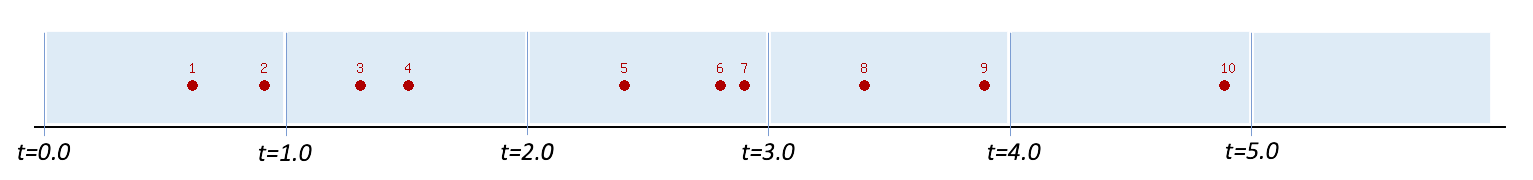
\includegraphics[width=0.8\textwidth]{img/descarga (2).png}
    \end{figure}
    \begin{itemize}
        \item ALOHA
        \begin{itemize}
            \item\textbf{Suppose all nodes are implementing the Aloha protocol. For each message, indicate the time at which each transmission begins}
            The answer is: 0.6,0.9,1.3,1.5,2.4,2.8,2.9,3.4,3.9,4.9.
            \item\textbf{Which messages transmit succesfully?} The answer is: 10.
        \end{itemize}
        
        \item SLOTTED-ALOHA
        \begin{itemize}
            \item\textbf{Suppose all nodes are implementing the Slotted Aloha protocol. For each message, indicate the time at which each transmission begins}
            The answer is: 1,1,2,2,3,3,3,4,4,5.
            \item\textbf{Which messages transmit succesfully?} The answer is: 10.
        \end{itemize}
        
        \newpage
        \item CSMA
        \begin{itemize}
            \item\textbf{Suppose all nodes are implementing Carrier Sense Multiple Access (\textit{CSMA}), but whitout collision detection. Suppose that the time
            from when a message transmission begins until it is beginning to be received at other nodes is 0.4 time units. (\textit{Thus if a node begins 
            transmitting a message at t=2.0 and transmits that message until t=3-0, then any node performing carrier sensing in the interval [2.4, 3.4] will 
            sense the channel busy.}) For each message, indicate the time at which each message transmission begins, or indicate that messge transmission does not
            begin due to a channel that is sensed busy when that message arrives.}
            The answer is: 0.6,0.9,s,s,2.4,s,s,s,3.9,s.
            \item\textbf{Which messages transmitted succesfully?} The answer is: 5, 9.
        \end{itemize}
        
        \item CSMA-CD
        \begin{itemize}
            \item\textbf{Suppose all nodes are implementing Carrier Sense Multiple Access (\textit{CSMA}), with collision detection (\textit{CSMA/CD}). Suppose that
            the time from when a message transmission begins until it is beginning to be received at other nodes is 0.4 time units, and assume that a node can stop transmission
            instantaneously when a message collision is detected. (\textit{Thus if a node begins transmitting a message at t=2.0 and transmits that message until t=3.0, then
            any node performing carrier sensing in the interval [2.4, 3.4] will sense the channel busy.)} For each message, indicate the time at which each message
            transmission begins, or indicate that message transmission does not begin due to a channel that is sensed busy when that message arrives.}
            The answer is: 0.6,0.9,s,s,2.4,s,s,s,3.9,s.
            \item\textbf{Which messages transmit succesfully?} The answer is: 5, 9.
        \end{itemize}
    \end{itemize}
